\documentclass[]{article}
\usepackage{lmodern}
\usepackage{amssymb,amsmath}
\usepackage{ifxetex,ifluatex}
\usepackage{fixltx2e} % provides \textsubscript
\ifnum 0\ifxetex 1\fi\ifluatex 1\fi=0 % if pdftex
  \usepackage[T1]{fontenc}
  \usepackage[utf8]{inputenc}
\else % if luatex or xelatex
  \ifxetex
    \usepackage{mathspec}
    \usepackage{xltxtra,xunicode}
  \else
    \usepackage{fontspec}
  \fi
  \defaultfontfeatures{Mapping=tex-text,Scale=MatchLowercase}
  \newcommand{\euro}{€}
\fi
% use upquote if available, for straight quotes in verbatim environments
\IfFileExists{upquote.sty}{\usepackage{upquote}}{}
% use microtype if available
\IfFileExists{microtype.sty}{%
\usepackage{microtype}
\UseMicrotypeSet[protrusion]{basicmath} % disable protrusion for tt fonts
}{}
\usepackage[margin=3cm]{geometry}
\usepackage{listings}
\usepackage{graphicx}
\makeatletter
\def\maxwidth{\ifdim\Gin@nat@width>\linewidth\linewidth\else\Gin@nat@width\fi}
\def\maxheight{\ifdim\Gin@nat@height>\textheight\textheight\else\Gin@nat@height\fi}
\makeatother
% Scale images if necessary, so that they will not overflow the page
% margins by default, and it is still possible to overwrite the defaults
% using explicit options in \includegraphics[width, height, ...]{}
\setkeys{Gin}{width=\maxwidth,height=\maxheight,keepaspectratio}
\ifxetex
  \usepackage[setpagesize=false, % page size defined by xetex
              unicode=false, % unicode breaks when used with xetex
              xetex]{hyperref}
\else
  \usepackage[unicode=true]{hyperref}
\fi
\hypersetup{breaklinks=true,
            bookmarks=true,
            pdfauthor={Marco Wettstein},
            pdftitle={Timetraces Seminararbeit Handheld},
            colorlinks=true,
            citecolor=blue,
            urlcolor=blue,
            linkcolor=magenta,
            pdfborder={0 0 0}}
\urlstyle{same}  % don't use monospace font for urls
\setlength{\parindent}{0pt}
\setlength{\parskip}{6pt plus 2pt minus 1pt}
\setlength{\emergencystretch}{3em}  % prevent overfull lines
\setcounter{secnumdepth}{5}

\title{Timetraces Seminararbeit Handheld}
\author{Marco Wettstein}
\date{}
%%%%%%%%%%%%%%%%%%%%%%%%%%%%%%%%%%%%%%%%%%%%%%%%%%%%%%%%%%%%%%%%%
%  _____   ____  _____                                          %
% |_   _| /  __||  __ \    Institute of Computitional Physics   %
%   | |  |  /   | |__) |   Zuercher Hochschule Winterthur       %
%   | |  | (    |  ___/    (University of Applied Sciences)     %
%  _| |_ |  \__ | |        8401 Winterthur, Switzerland         %
% |_____| \____||_|                                             %
%%%%%%%%%%%%%%%%%%%%%%%%%%%%%%%%%%%%%%%%%%%%%%%%%%%%%%%%%%%%%%%%%
%
% Project     : LaTeX doc Vorlage für Windows ProTeXt mit TexMakerX
% Title       : 
% File        : header.tex Rev. 00
% Date        : 23.4.12
% Author      : Remo Ritzmann
% Feedback bitte an Email: remo.ritzmann@pfunzle.ch
%
%%%%%%%%%%%%%%%%%%%%%%%%%%%%%%%%%%%%%%%%%%%%%%%%%%%%%%%%%%%%%%%%%

%\documentclass[twoside,10pt,parskip=half,ngerman]{scrreprt}

%***********************************************************************
% include some libs
%***********************************************************************
\usepackage[utf8]{inputenc}
\usepackage{listings}
\usepackage{color}
\usepackage{fancyhdr}
\usepackage{rotating}
\usepackage{titlesec}
\usepackage{mathptmx}
% \usepackage{helvet}
\usepackage[scaled]{uarial}
\renewcommand*\familydefault{\sfdefault} %% Only if the base font of the document is to be sans serif
\usepackage[T1]{fontenc}
\usepackage{ngerman}
\usepackage{textcomp}
\usepackage[squaren]{SIunits}
\usepackage{graphicx}
\usepackage{url}
\usepackage{geometry}
\usepackage[absolute]{textpos}
\usepackage{makeidx}
\usepackage{colortbl}
\usepackage{pdflscape}
\usepackage{pdfpages}
\usepackage{tabularx}
\usepackage{lmodern}
\usepackage{longtable}
\usepackage{array}
\usepackage{float}
\usepackage{scrhack}
\usepackage{wallpaper} %\ThisTileWallPaper{}
\usepackage[super,square]{natbib} %für BibTeX Literaturverzeichnis




%***********************************************************************
% various styles
%***********************************************************************	

%create index
\makeindex

%define pagestyle
\pagestyle{fancy}

%use sans-serif font 
%\renewcommand{\familydefault}{\sfdefault}

%define page margin
\geometry{a4paper, top=30mm, left=30mm, right=30mm, bottom=30mm,headsep=10mm,footskip=10mm}

%textpos parameter
\setlength{\TPHorizModule}{30mm}
\setlength{\TPVertModule}{\TPHorizModule}
\textblockorigin{10mm}{10mm} % start everything near the top-left corner
\setlength{\parindent}{0pt}

%horizontal lines for titlepage 
\newcommand{\HRule}{\rule{\linewidth}{0.5mm}}

%reference to source items inlc source number
\newcommand{\srcref}[1]{\nameref{src:#1} \cite{#1}}

%header / footer 
\renewcommand{\headrulewidth}{0.3pt}
\renewcommand{\footrulewidth}{0.3pt}

\fancyhead[LO,RE]{} %clear headings for contents 
\fancyhead[RO,LE]{\nouppercase{\rightmark}} %right odd pages and left even pages
\fancyhead[LO,RE]{\MakeUppercase{\leftmark}} %left odd pages and right even pages
\fancyfoot[LE,RO]{\thepage} %page numbering
\fancyfoot[C]{} %clear centered page numbering 

%define some colors
\definecolor{gray}{rgb}{0.95,0.95,0.95}
\definecolor{darkgray}{rgb}{0.4,0.4,0.4}
%listing colors
\definecolor{lgray}{RGB}{250,250,250}
\definecolor{lgreen}{RGB}{63,127,95}
\definecolor{lred}{RGB}{127,0,85}
\definecolor{lblue}{RGB}{42,0,255}

%***********************************************************************
% listing
%***********************************************************************

\lstset{		
		basicstyle=\small\ttfamily,
		frame=single,
		numbers=left,	
		numberstyle=\tiny,
		%firstnumber=auto,
		numberblanklines=true,
		captionpos=b,
		extendedchars=true,
		float=ht,
		showtabs=false,
		tabsize=2,
		showspaces=false,
		showstringspaces=false,
		breaklines=true,
		%prebreak=\Righttorque,
		backgroundcolor=\color{lgray},
		keywordstyle=\color{lred}\bfseries, 
		commentstyle=\color{lgreen}\ttfamily,
%		morekeywords={printstr, printhexln},
		stringstyle=\color{lblue},
		xleftmargin=0.5cm,
		xrightmargin=0.5cm
}

\lstloadlanguages{C++}

%\lstdefinelanguage{xc}{
%     keywords={printstr, printhexln, attributes, class, classend, do, empty, endif, endwhile, fail, function, functionend, if, implements, in, inherit, inout, not, of, operations, out, return, set, then, types, while, use},
%     keywordstyle=\color{lred}\bfseries,
%     ndkeywords={},
%     ndkeywordstyle=\color{yellow}\bfseries,
%     identifierstyle=\color{black},
%     sensitive=false,
%     comment=[l]{//},
%     commentstyle=\color{lgreen}\ttfamily,
%     string=[l]{"},
%     stringstyle=\color{lblue}\ttfamily
%  }

\begin{document}
\maketitle

{
\hypersetup{linkcolor=black}
\setcounter{tocdepth}{3}
\tableofcontents
}
\listoffigures

\lstlistoflistings

\newpage

\section{Vorwort}\label{vorwort}

Sehr geehrte Leserschaft

Smartphones und andere mobilen Geräte haben nicht nur durch ihre
Mobilität unseren Alltag und die Arbeitswelt erobert, sondern auch durch
neue Bedienkonzepte und durch Bündelung verschiedener Datenquellen und
Dienste. Kalender und GPS verbinden Ort und Zeit des Benutzers - das
Gerät weiss jederzeit, was der Benutzer gerade tut oder geplant hat und
wo er sich befindet und kann daraus Absichten des Benutzers vorhersehen.
Konzepte wie Google Now verfolgen diesen Ansatz \cite{googleNow}. Das
Smartphone wird vermehrt zum intelligenten digitalen Assistenten.

Mit dieser Vision versuchte ich die firmeninterne Anwendung zur
Zeiterfassung (``controllr'') für Smartphones neu zu konzipieren.

Die bestehende Anwendung funktioniert prinzipiell auch auf mobilen
Endgeräten mit kleinen Bildschirmen mittels einfachen Verfahren des
Responsive Webdesign\footnote{Prinzipell werden beim Responsive
  Webdesign Elemente auf einer Webseite so angeordnet und allenfalls in
  ihrer Grösse angepasst, sodass sie auf verschiedenen Bildschirmgrössen
  und -formate sinnvoll Platz haben. (``Responsive Webdesign -
  Wikipedia'')}, doch reicht das reine Umordnen der Elemente in diesem
Fall nicht, um den Prozess der Zeiterfassung sinnvoll auf ein Smartphone
zu übertragen. Denn nicht nur die Grösse des Bildschirms hat einfluss
auf die Bedienbarkeit, sondern auch die Eingabemöglichkeiten des
Gerätes. Schaltflächen sind mit einem berührungssensitiven Bildschirms
schwerer zu treffen und müssen entsprechend gestaltet werden, ebenso ist
die Eingabe von Text auf einem Smartphone aufwendiger und daher
langsamer im Vergleich zu einem klassischen Computer mit Maus und
Tastatur.

Um dieses Problem anzugehen überlegte ich mir daher zwei
Stossrichtungen:

\begin{itemize}
\itemsep1pt\parskip0pt\parsep0pt
\item
  Bedienelemente der Zeiterfassung für Smartphones optimieren
\item
  Die Menge der Bedienelemente und Eingaben reduzieren
\end{itemize}

Während die erste Option in der Regel einfacher umzusetzen ist und auch
häufig gemacht wird, empfinde ich doch die zweite Variante als weitaus
spannender und zeitgemässer.

Mit der Eingangs erwähnten Vision im Hinterkopf überlegte ich mir daher,
wie ich die Anzahl Benutzerinteraktionen für eine Zeiterfassung
minimieren kann, indem ich verschiedene Datenquellen eines Mitarbeiters
miteinander verbinde.

\newpage

\section{Ist-Analyse}\label{ist-analyse}

\subsection{Ausgangslage}\label{ausgangslage}

Jeder Mitarbeiter muss regelmässig seine gearbeitete Zeit in der
Anwendung ``Controllr'' eintragen. Dabei wird unter anderem die
gearbeitete Zeit, das zugehörige Projekt, ein Task-Typ und eine
Beschreibung angegeben.

Diese Tasks müssen am Ende eines Monats bestätigt werden, damit eine
Auswertung stattfinden kann.

Die Anwendung ist als Webbasierte Lösung implementiert und ist für die
Benutzung am Computer ausgerichtet, funktioniert prinzipiell aber auch
auf kleineren Smartphones und Tablet-Computer. Dabei wurden die Elemente
bei wenig Platz untereinander angeordnet. Die Eingabe-Elemente bleiben
unangetastet.

Die Erfassung eines Zeiteintrages erfordert folgende Interaktionen:

\begin{itemize}
\itemsep1pt\parskip0pt\parsep0pt
\item
  Auswahl eines Tages durch klick auf einen kleinen Kalender.
\item
  Auswahl eines Projektes durch ein \emph{Select}-Element
\item
  Auswahl eines Tasks durch ein \emph{Select}-Element
\item
  Eingabe der Startzeit im Format hh:mm
\item
  Eingabe der Endzeit im Format hh:mm
\item
  Eingabe eines Beschreibungstextest
\item
  Bestätigung durch Klick auf ``Create Entry''
\end{itemize}

Weitere Einzelheiten sind unter Abschnitt \ref{secControllr} zu finden.

Jedem Mitarbeiter stehen weitere Systeme zur Verfügung, welche er in
seiner täglichen Arbeit benutzen kann (Siehe Abschnitt
\ref{secSysteme}). Vieler dieser Systeme können ausgewertet werden um
Kontext-Daten eines Benutzers zu TODO\ldots{}

\subsection{Rollen}\label{rollen}

Ein zentraler Aspekt der Arbeit sind die erwähnten Kontext-Daten der
Benutzer, doch nicht jeder Mitarbeiter hat die gleiche Art von Kontext.
Ein Entwickler ``dokumentiert'' seine Arbeit häufig in einer
Code-Versionisierungs-Software, für einen Projektleiter jedoch stehen
vielleicht Meetings und entsprechende Kalender-Einträge im Vordergrund.
Eine vorgängige Analyse der Rollen und verfügbaren Systemen ist daher
unabdingbar.

Nachfolgend eine Liste der Rollen, welche bei Panter vertreten sind.
Manche Mitarbeiter nehmen mehrere Rollen ein. Manche Mitarbeiter
arbeiten zudem häufig extern bei Kunden und nutzen teilweise andere
Systeme. Software-Engineer Konzipiert, erstellt, testet und wartet
Anwendungen und Systeme. Arbeitet häufig im Team in einem agilen
Entwicklungsprozess (häufig Scrum).

\begin{description}
\itemsep1pt\parskip0pt\parsep0pt
\item[Scrum-Master]
Leitet und überwacht den Scrumprozess. Er plant und moderiert häufig die
Scrum-Meetings, wie Planning-Meeting und Daily Scrum-Meetings, sowie
andere Scrum-Aktivitäten.
\item[Product Owner-Assistent]
Der Product Owner-Assistent (PO-Assistant) wird dem häufig externen
Product Owner zur Seite gestellt und unterstützt diesen beim Erstellen
und Abnehmen der User Stories.
\item[Sales]
Sales-Mitarbeiter beraten bestehende Kunden und potentielle neue Kunden
über neue Projekte und nehmen an Pitches teil.
\item[Administration]
Kümmert sich um Buchhaltung, Administation und Human Resources-Aufgaben.
\item[Marketing]
Erstellt und setzt das Marketing-Konzept der Firma um, fördert die
Sichtbarkeit der Firma und unterstützt dadurch die Bestrebungen der
Sales-Mitarbeiter.
\item[Community-Manager]
Kümmert sich um die Verwaltung des Cowork-Space ``colab-zurich.ch''. Zur
Zeit (Ende 2014) eine Praktikumsstelle.
\end{description}

\pagebreak

\subsection{\texorpdfstring{Systeme\label{secSysteme}}{Systeme}}\label{systeme}

Den Mitarbeitern stehen in der Regel folgende Systeme und Anwendungen
zur Verfügung, sofern sie nicht im externen Einsatz eingschränkt sind:

\subsubsection{\texorpdfstring{Controllr\label{secControllr}}{Controllr}}\label{controllr}

Von Panter erstellte Software für das Finanz-Controlling, Zeiterfassung
und Resourcenplanung. Es ist das zentrale System, welches die Anwendung
anbinden soll. Zugriff erfolgt über ein Webinterface oder über eine
REST-Schnittstelle.

\begin{figure}[htbp]
\centering
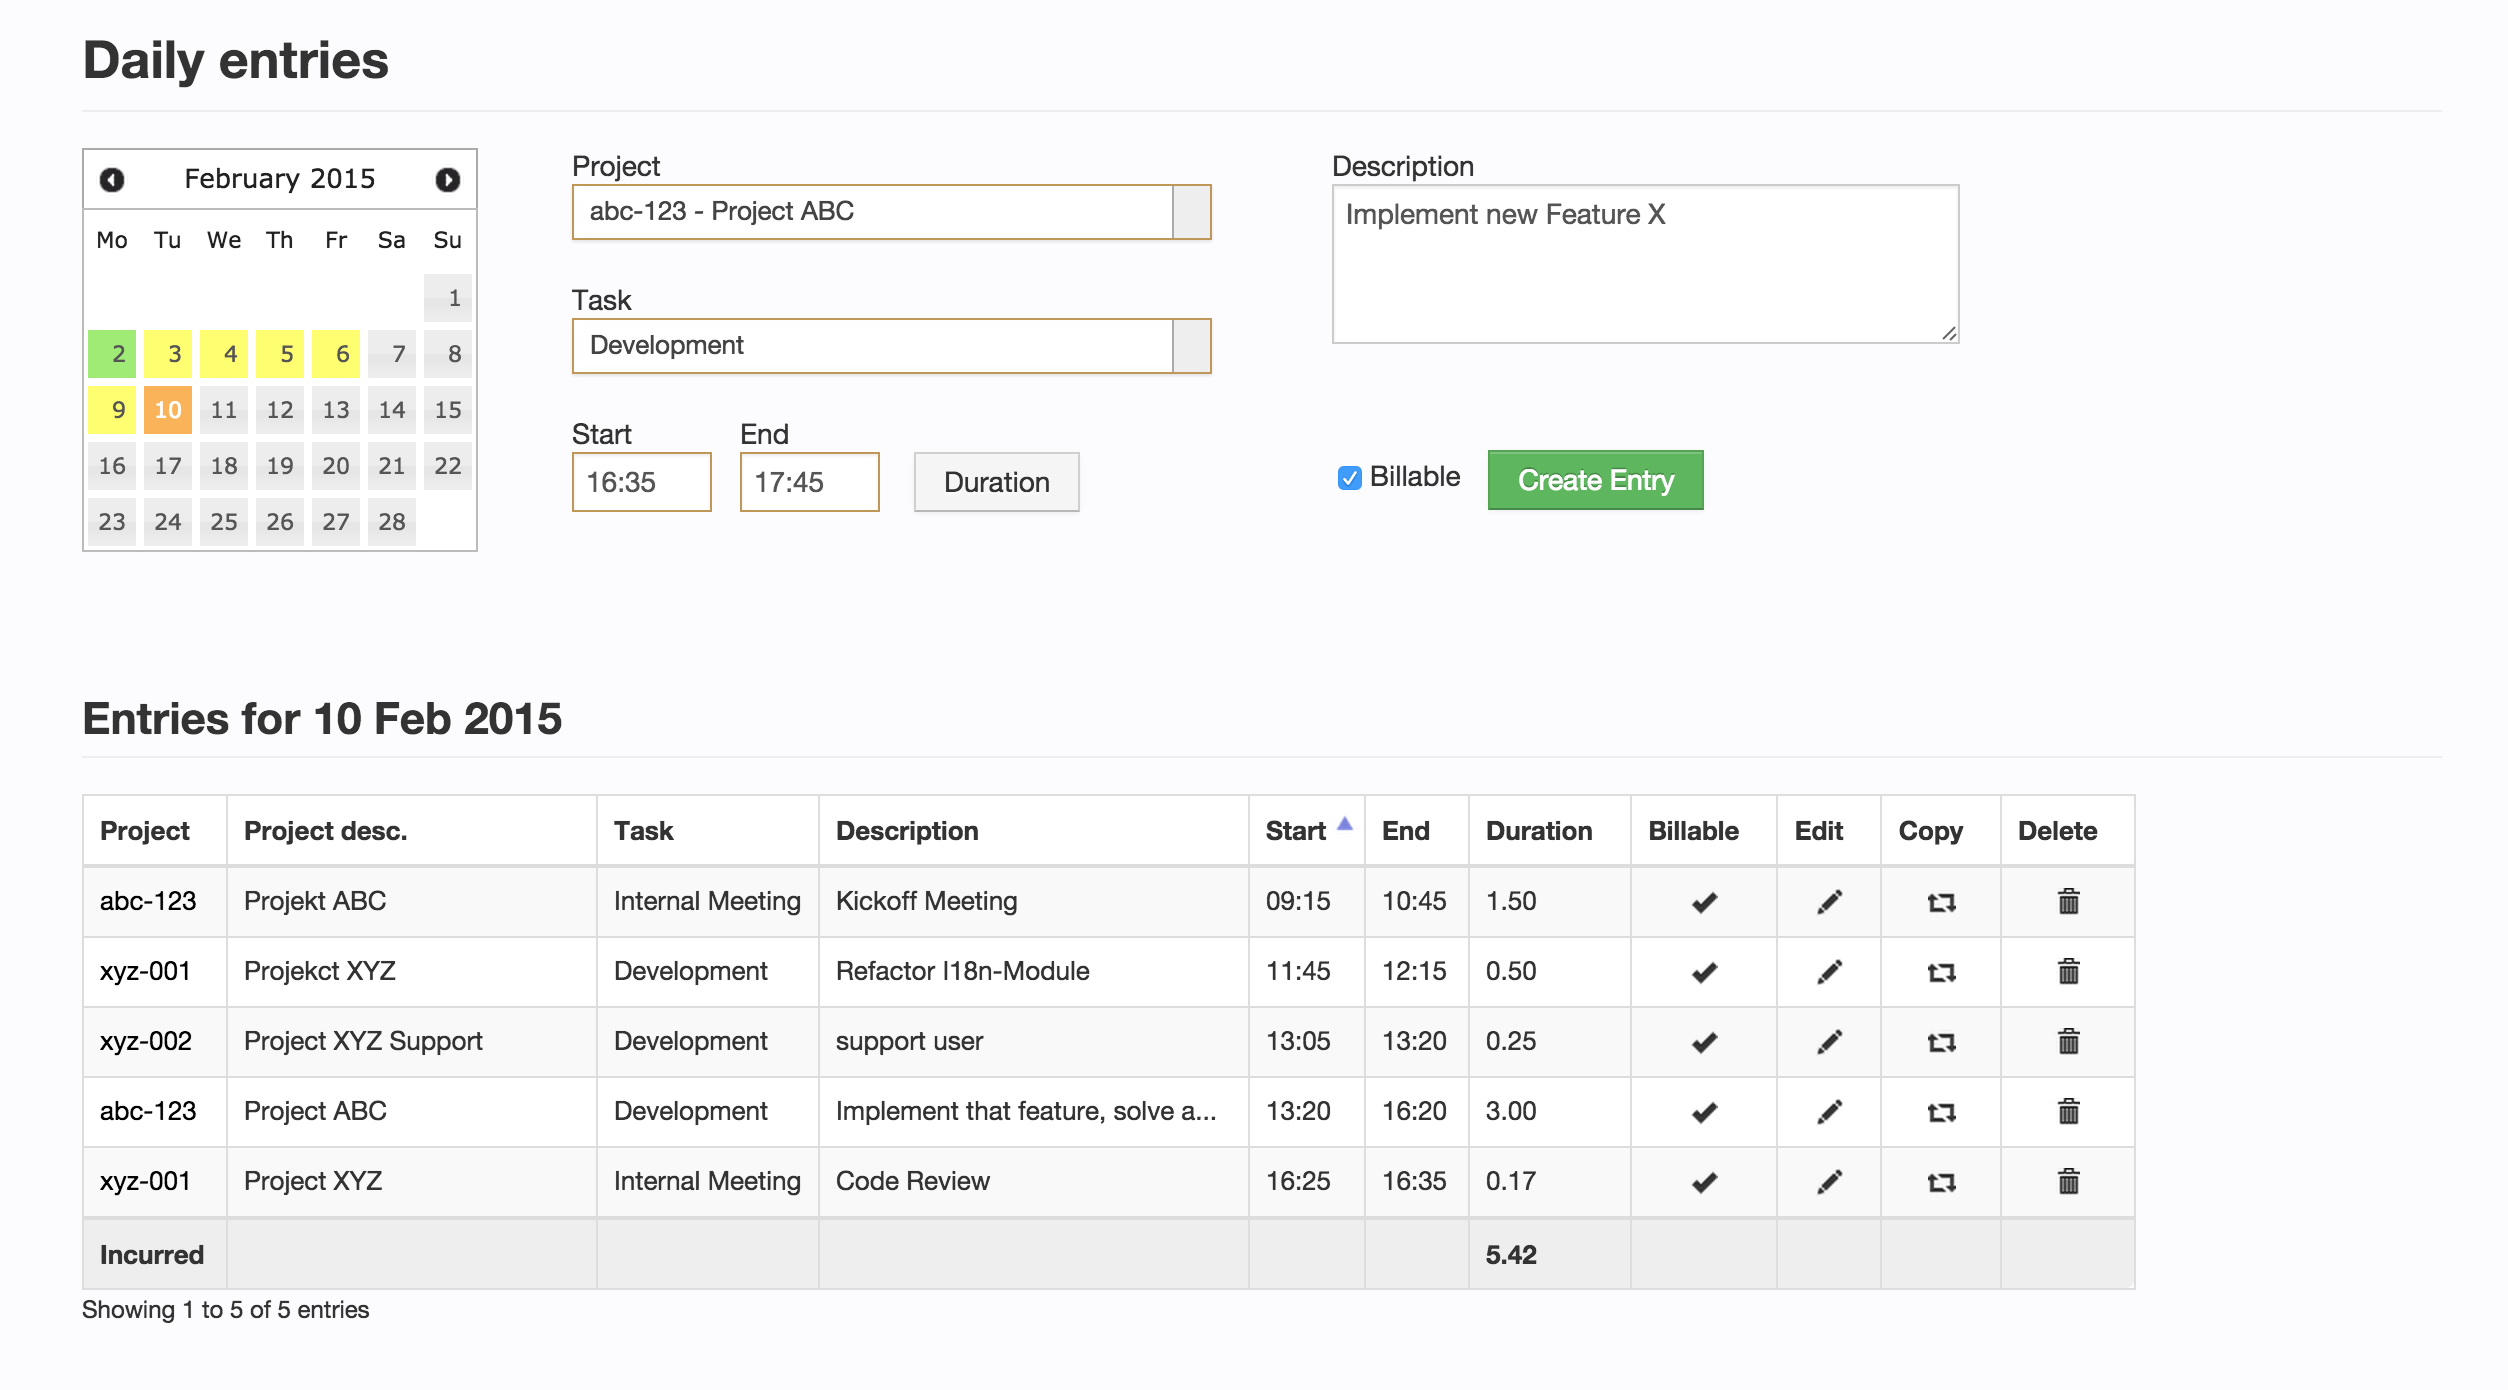
\includegraphics{../img/controllr.png}
\caption{Screenshot von ``Controllr''\label{figControllr}}
\end{figure}

\paragraph{Zeiteinträge}\label{zeiteintruxe4ge}

Die REST-Schnittstelle von Controllr ermöglicht unter anderem das Lesen
und Manipulieren von Zeiteinträgen, Projekten und Tasks. Im Listing
\ref{lstcontrollrentries} sind die Schnittstellen zu den Zeiteinträgen
zu sehen. Diese Schnittstellen dienen zum Lesen (GET), Erstellen (POST),
Bearbeiten (PUT / PATCH) und Löschen (DELETE) von Zeiteinträgen. Listing
\ref{lstcontrollrentriesresult} zeigt das Schema eines solchen
Zeiteintrages.

\begin{lstlisting}[caption=Controllr REST API für Zeiteinträge, label=lstcontrollrentries]
GET      /api/entries(.:format)                          
POST     /api/entries(.:format)                          
GET      /api/entries/new(.:format)                      
GET      /api/entries/:id/edit(.:format)                 
GET      /api/entries/:id(.:format)                      
PATCH    /api/entries/:id(.:format)                      
PUT      /api/entries/:id(.:format)                      
DELETE   /api/entries/:id(.:format)
\end{lstlisting}

\begin{lstlisting}[caption=Schema von /api/entries, label=lstcontrollrentriesresult]
{
    "id": 12513,
    "created_at": "2014-09-15T14:25:07.000Z",
    "updated_at": "2014-11-13T14:45:31.000Z",
    "deleted_at": null,
    "day": "2014-09-15",
    "start": "2000-01-01T09:50:00Z",
    "end": "2000-01-01T10:00:00Z",
    "duration": 10,
    "state": "invoiced",
    "description": "Standup Meeting",
    "billable": true,
    "invoice_id": 123,
    "project_id": 1100,
    "task_id": 10042,
    "user_id": 12,
    "project_shortname": "abc-001",
    "task_name": "Internal Meeting",
    "user_username": "maw"
}
\end{lstlisting}

Auffallend ist ``start'' und ``end'', bei denen das Datum offenbar aus
Formatgründen angefügt wird und ohne Relevanz ist. Lediglich die Zeit
ist relevant. Für das Datum des Zeiteintrages ist ``day'' relevant. Dies
bedeutet auch, dass jeder Zeiteintrag einem Tag zugeordnet ist, es kann
keine einzelnzen Zeiteinträge geben, die über mehrere Tage gehen (z.b.
über Mitternacht).

Manche relationale Daten sind zudem Denormalisiert (project\_shortname
und task\_name).\footnote{Als Denormalisierung bezeichnet man das
  bewusste Einfügen redundanter Informationen einer relationalen
  Datenbank zu Gunsten eines besseren Laufzeitverhaltens oder
  einfacherem Zugriff. Im obigen Beispiel, wird neben der project\_id
  auch der project\_shortname mitgegeben, welcher direkt abhängig von
  der project\_id ist. Das Denormalisieren entspricht der Umkehrung der
  Normalisierung.}

Der Lesezugriff (GET) auf diese Daten liefert jeweils ein Array dieser
Einträge. Mit GET-Parameter können die Resultate gefiltert werden:

\begin{description}
\itemsep1pt\parskip0pt\parsep0pt
\item[date\_to, date\_from]
Liefert die Einträge mit ``day'' zwischen date\_from und date\_to
(inklusive)
\item[employee\_usernames]
Liefert nur die Einträge eines bestimmten Users
\item[project\_shortnames]
Liefert nur die Einträge eines bestimmten Projektes
\item[states]
Liefert nur Einträge mit einem bestimmten state
\end{description}

\paragraph{Projekte}\label{projekte}

Projekte können über die Schnittstellen von Listing
\ref{lstControllrProjects} abgerufen werden und liefern ein Array von
Projekten wie im Schema \ref{lstcontrollrProjectsResult}

\begin{lstlisting}[caption=Controllr REST API für Projekte, label=lstControllrProjects]
GET      /api/projects(.:format)                         
GET      /api/projects/:id(.:format)   
\end{lstlisting}

\begin{lstlisting}[caption=Schema von /api/projects, label=lstcontrollrProjectsResult]
{
    "id": 1234,
    "shortname": "abc-001",
    "description": "Beispiel Projekt",
    "start": "2014-03-21",
    "end": "2014-11-13",
    "created_at": "2014-04-07T10:15:11.000Z",
    "updated_at": "2015-02-06T17:50:39.000Z",
    "project_state_id": 6,
    "probability": "1.0",
    "deleted_at": null,
    "external": true,
    "note": "Dies ist ein Beispielprojekt",
    "worktime_budget": "1302.0",
    "cached_expected_profitability": 0.581247,
    "cached_expected_return": 685.5,
    "company_id": 111,
    "active": true,
    "leader_id": 62,
    "business_unit_id": 1,
    "cached_budget": "112236.0",
    "budget_notification_sent": false,
    "mwst": true,
    "daily_rate": "1200.0",
    "hours_per_day": "8.0",
    "google_id": "Gyqrt64o8AOywyeBGyqrt64o8AOywyeB",
    "planning_note": "",
    "time_billable": "1255:43",
    "burned_time": "1301:47"
}
\end{lstlisting}

\paragraph{Tasks}\label{tasks}

Die Tasks-Schnittstelle wird in Listings \ref{lstControllrTasks} und
\ref{lstcontrollrTasksResult} beschrieben.

Es existieren noch weitere Schnittstellen, welche aber für die Arbeit
weniger relevant sind.

\begin{lstlisting}[caption=Controllr REST API für Tasks, label=lstControllrTasks]
GET      /api/tasks(.:format)                            
GET      /api/tasks/:id(.:format)   
\end{lstlisting}

\begin{lstlisting}[caption=Schema von /api/tasks, label=lstcontrollrTasksResult]
{
    "id": 6711,
    "name": "Freelance vor Ort",
    "project_id": 3330,
    "created_at": "2011-11-24T19:02:08.000Z",
    "updated_at": "2011-11-24T19:07:23.000Z",
    "active": true,
    "deleted_at": null,
    "billable_by_default": true,
    "worktime_budget": null,
    "global_task_id": null,
    "daily_rate": null
}
\end{lstlisting}

\paragraph{Authentifizierung}\label{authentifizierung}

Für die Authenfizierung des Users muss ein Token (user\_token) an die
Schnittstellen mitgegeben werden. Der Token kann auf der Profil-Seite im
Controllr abgefragt werden, nachdem man sich eingeloggt hat.

\subsubsection{Google Apps}\label{google-apps}

Für Email, Kalender und Dateien wird Googles Business Angebot ``Google
Apps'' verwendet. Der Service kann über verschiedene REST-APIs abgefragt
und bedient werden. Da Implementationen dieser Schnitstellen in vielen
Sprachen bereits existieren, bietet es sich an, manche dieser
Schnittstellen zu verwenden.

\paragraph{Email}\label{email}

Business-Variante von Googles Mail-Lösung GMail. Die Anwendung wird im
Browser bedient und kann zudem über eine REST-API abgefragt werden. Es
können insbesondere Nachrichten, Threads (Zusammengehörende Nachrichten)
und Labels abgefragt werden. Siehe (``Google Apps Email API'').

Möglich wäre beispielsweise, Nachrichten nach Projekt-Namen aus
``Controllr'' zu durchsuchen und diese als Quelle zu verwenden.

\paragraph{Kalender}\label{kalender}

Kalender-Anwendung von Google. Wird in der Firma häufig verwendet und
kann ebenfalls über eine REST-API abgerufen weren. Kalendereinträge
bieten sich insbesondere an, da diese bereits über ein ähnliches Format
verfügen wie die Zeiteinträge; sie haben u.a. eine Start- und Endzeit,
sowie eine Beschreibung. (``Google Kalender API'').

\paragraph{Authentifizierung}\label{authentifizierung-1}

Die Authentifizierung wird OAuth 2.0 verwendet. Es existieren zahlreiche
Implementierungen dieses Standards, was die Verwendung dieser
Schnittstellen vereinfacht. (``Google OAuth2'')

\subsubsection{Redmine}\label{redmine}

Projektverwaltungs-Anwendung, welche von der Firma für viele Projekte
verwendet wird. Die Projekte werden stets in einem agilen Prozess
entwickelt, welcher meistens SCRUM ist. In Redmine befinden sich daher
Stories und zugehörige Tasks, sowie deren Stand. Mitarbeiter, welche an
externen Projekten beim Kunden arbeiten, verwenden allerdings häufig
nicht Redmine, sondern jeweilige Firmen-Interne Anwendungen.

Redmine bildet nicht direkt typische SCRUM-Artefakte wie Stories und
Tasks ab, sondern es werden üblicherweise ``Issues'' erfasst. Über
Erweiterungen können aber Stories und Tasks ebenfalls erfasst werden,
diese werden dann als unterschiedliche ``Issue''-Typen erfasst.

Redmine bietet ebenfalls eine REST-API, welche es u.a. erlaubt, Issues
und Projekte abzufragen. (``Redmine REST API'')

\paragraph{Authentifizierung}\label{authentifizierung-2}

Für die Authentifizierung muss ein fester Token mitgegeben werden,
welcher User-spezifisch ist und auf der Profil-Seite von Redmine
abgefragt werden kann.

\subsubsection{Github}\label{github}

Verwaltungsoberfläche und Hosting-Dienst für Software-Projekte, welche
die namensgebende Quellcode-Versionsverwaltungs-Software git verwendet.
Nicht alle Projekte verwenden Github für die Quellcode-Versionisierung.
Insbesondere externe Projekte beim Kunden verfügen über eigene
Versionisierungstools.

Github verfügt ebenfalls über reichhaltige REST-APIs; die Beschreibung
dieser APIs kann in der Quellenangabe eingesehen werden. Es bietet sich
an, die Schnittstelle ``Events'' zu verwenden, welche beispielsweise
Aktivitäten eines Benutzers aufzeigt. Damit kann die Tätigkeit eines
Users auf Github an einem Tag abgefragt werden. Die Art der Aktivität
und das Repository sind dabei zweitrangig.
(https://developer.github.com/v3/)

Ein solches Event verfügt über einen Typ, eine Beschreibung, eine
Identifizerung des Repositories und einen Zeitpunkt, an dem dieses
Ereignis oder Aktivität stattgefunden hat.

\paragraph{Authentifizierung}\label{authentifizierung-3}

Github unterstützt verschiedene Authentifizierungsverfahren: Basic
Authentication mit Username / Password, OAuth2 mit Token oder OAuth2 mit
Key/Secret , siehe (``Github Authentifizierung'').

\subsubsection{Timetunnel}\label{timetunnel}

Der Timetunnel ist eine von Panter entwickelte Software, welche es
ermöglicht, Zeiteinträge direkt über den Kalender zu tätigen. Die
Software besteht im wesentlichen aus einem Script. welches
Kalendereinträge mit definierten Stichworten im Titel sucht und als
Zeiteinträge für die Zeiterfassung in Controllr erfasst. Das bedeutet,
Zeiteinträge können direkt im Kalender erfasst, statt im Web-GUI. Die
Anwendung wird nach erster Abklärung kaum genutzt, allerdings können
Ideen davon, wie z.b. das Tagging der Einträge wiederverwendet werden.

\subsubsection{strms.io (vormals
storyline.li)}\label{strms.io-vormals-storyline.li}

Sich in Entwicklung befindende Software, welche von Panter entwickelt
wird. Die Anwendung konsolidiert verschiedene Google-Dienste wie Email,
Kalender und Google Drive und stellt die Aktivitäten eines Benutzers auf
diesen Diensten chronologisch dar. Ziel ist es, Emails, Kalendereinträge
und Dateien in einen Zusammenhang zu bringen. Die Anwendung bietet sich
als Datenquelle an, weil sie bereits mehrere Quellen vorkonsolidiert und
chronologisch ordnet. Das Projekt befindet sich zum Zeitpunkt dieser
Arbeit in Entwicklung. Eine Zusammenarbeit, sowie Wissensaustausch ist
möglich. Es existieren allerdings zum Zeitpunkt der Entwicklung dieser
Arbeit keine Schnittstellen, welche einen programmatischen Zugriff
erlauben.

\subsubsection{Systemübersicht}\label{systemuxfcbersicht}

Abbildung \ref{figSystems} zeigt eine Übersicht der Syteme und eine
mögliche Integration der zu erstellenden Applikation.

\begin{figure}[htbp]
\centering
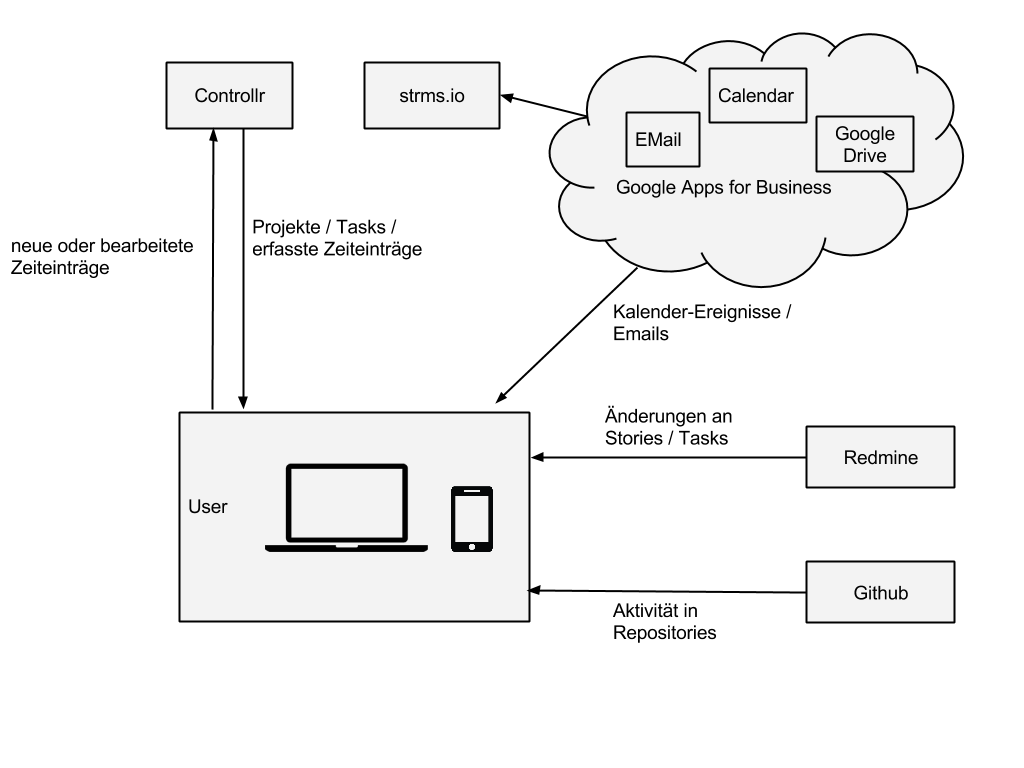
\includegraphics{../img/systems.png}
\caption{Systemübersicht\label{figSystems}}
\end{figure}

\newpage

\section{Anforderungsanalyse}\label{anforderungsanalyse}

Um das Nutzungsverhalten der verschiedenen Systeme zu erruieren, wurde
eine Umfrage unter den Mitarbeitern gemacht.

Es ging darum, einen Einblick in folgende Fragestellungen zu erhalten:

\begin{itemize}
\itemsep1pt\parskip0pt\parsep0pt
\item
  Welche Systeme werden wie oft verwendet?
\item
  Welche Systeme protokollieren die Arbeit der Mitarbeiter am besten?
\item
  Gibt es Unterschiede zwischen verschiedenen Rollen oder Mitarbeiter im
  internen und Mitarbeiter im externen Einsatz?
\item
  Wird die Zeiterfassung regelmässig gemacht oder unregelmässig?
\item
  Wo liegen die Probleme der bestehenden Lösung?
\item
  Welche Smartphone-Betriebsysteme werden verwendet?
\item
  Würde eine Smartphone-App auf Anklang stossen?
\end{itemize}

\subsection{Resultate}\label{resultate}

In der Auswertung der Umfrage wurden folgende Beobachtungen gemacht: -
Google Kalender und Email wird von jedem Mitarbeiter häufig verwendet,
egal ob im externen Einsatz oder nicht. - Github und Redmine werden
ebenfalls sehr häufig verwendet, einen signifikanten Unterschied
zwischen internen oder externen Einsatz wurde nicht festgestellt,
allerdings waren nur sehr wenige Beantwortungen von externen
Mitarbeitern eingegangen. - Die Mitarbeiter schätzen, dass Redmine,
Github, Email und Kalender ihre tägliche Arbeit am besten
protokollieren, wobei der Kalender leicht vorne liegt. - Die
Zeiterfassung wird häufig am Abend nach einem Arbeitstag gemacht. - Die
Zeiteinträge werden generell nicht allzu detailiert kommentiert. - Viele
Mitarbeiter arbeiten an mehreren Projekten täglich, manche aber auch nur
an einem pro Tag. Bei dieser Frage, die mit einer Bewertung von 1-5
beantwortet werden musste, gab es zwei Häufungen mit wenig
Beantwortungen im Mittelfeld. Offenbar gibt es zwei Gruppen von
Mitarbeiter: Mitarbeiter die häufig nur an einem Projekt arbeiten und
Mitarbeiter, welche häufig die Projekte wechseln. - Der Frage, ob eine
Mobile-App von den Mitarbeitern genutzt werden würde, wurde von einer
Mehrheit mit Ja beantwortet, allerdings haben immerhin 30\% der
Mitarbeitern die Frage verneint. In den Kommentaren hat sich dann
gezeigt, dass diese eine Lösung bevorzugen würden, die auch am Computer
funktioniert und nicht an ein Smartphone gebunden ist. - Android und IOS
wird von ähnlich vielen Mitarbeitern genutzt, wobei Android etwas vorne
liegt. Andere Systeme kommen nicht zum Einsatz

\newpage

\section{Konzept}\label{konzept}

\subsection{Begriffe}\label{begriffe}

\begin{description}
\itemsep1pt\parskip0pt\parsep0pt
\item[Event]
Als ``Event'' wird in der Arbeit ein Ereignis mit einem bestimmten
Zeitpunkt, sowie Beschreibung und anderen Daten angesehen. Die
``Events'' der zu verwendenen Quellen, haben in der Regel keine
Zeitdauer und damit keine Start- und Endzeit, mit Ausnahme der Daten aus
dem Kalender. Ein Event kann im einfachen Fall ein Kalendereintrag sein.
Es kann aber auch ein Commit auf Github sein, ein abgeschlossener Task
auf Redmine oder ähnliches. Ein Event kann man damit auch als ``Spur''
(engl. ``Trace'') verstehen, die die tägliche Arbeit hinterlässt.
\item[Timeentry]
Unter ``Timeentry''\footnote{Einfache transkription aus dem Englischen
  von ``Zeiteintrag'' in Anlehnung an ``Entry'', dem Datenmodel, welches
  in der Zeiterfassungsapplikation ``Controllr'' verwendet wird} wird
ein zu erstellender Zeiteintrag auf der Zeiterfassungsapplikation
(Controllr) verstanden. Im Gegensatz zu einem ``Event'', verfügt ein
``Timeentry'' immer über eine Start- und eine Endzeit. Zudem wird einem
``Timeentry'' einem Projekt, einem Task und einem Datum zugewiesen und
mit Beschreibung und weiteren Metadaten versehen. Ein ``Timeentry''
entspricht also dem Modell eines geleisteten Stücks Arbeit, welches es
zu protokollieren gilt.
\end{description}

\subsection{Vom Event zum Timeentry}\label{vom-event-zum-timeentry}

Listet man alle gesammelten ``Events'' eines Tages nacheinander auf,
erhält man ein erstes Protokoll. Um daraus konkrete Zeiteinträge zu
erstellen, müssen die Events noch umgeformt und mit weiteren Daten
versehen werden:

\subsubsection{Projekt und
Task-zuweisung}\label{projekt-und-task-zuweisung}

Jedem Timeentry auf dem Controllr muss ein Projekt und ein Task
zugewiesen werden. Die Liste der Projekte und Tasks können von einer
Schnittstelle abgerufen werden. Jedes Projekt und jeder Task verfügt
über einen Namen und eine Beschreibung. Um für ein Event ein Task und
ein Projekt zu bestimmen, ergeben sich folgende Möglichkeiten:

\begin{itemize}
\itemsep1pt\parskip0pt\parsep0pt
\item
  Der Beschreibungstext und andere Metadaten des Events werden nach
  Projektnamen durchsucht und das entsprechende Projekt bei einem
  Treffer dem Event zugewiesen
\item
  Github-Events entsprechen i.d.R. einem ``Development''-Task
\item
  Kalendereinträge entsprechen einem ``Meeting''-Task
\item
  Der Enduser kann selbst Regeln bestimmen, beispielsweise indem er
  Schlüsselwörter definiert, welche ein bestimmtes Projekt oder einen
  bestimmten Task forcieren.
\end{itemize}

\subsubsection{Fehlende Start- und
Endzeit}\label{fehlende-start--und-endzeit}

Die Events aus den meisten Quellen besitzen aber nur einen Zeitpunkt,
keinen Start- und Endzeitpunkt. Es müssen also gewisse Annahmen
getroffen werden, um Start- und Endpunkt zu bestimmen. Folgende Annahmen
ergeben sich:

\begin{itemize}
\itemsep1pt\parskip0pt\parsep0pt
\item
  Der Zeitpunkt jedes Events entspricht dem Zeitpunkt, an dem eine
  Arbeit \textbf{beendet wurde}.

  \begin{itemize}
  \itemsep1pt\parskip0pt\parsep0pt
  \item
    In Hinblick auf Github-Commits trifft dies zu, da man i.d.R. nach
    einer Programmieraufgabe diese Änderungen in die Versionskontrolle
    speichert.
  \item
    Bei Redmine wird man häufig nach getaner Arbeit einen Task als
    Erledigt markieren oder den Progress des Tasks ändern
  \end{itemize}
\item
  Nach einem abgeschlossenen Task wendet man sich dem nächsten Task zu.
  Die \textbf{Startzeit eines Events} entspricht daher der
  \textbf{Endzeit des letzten Events}
\item
  Die \textbf{Startzeit des ersten Events an einem Tag} ist der übliche
  Arbeitsbeginn eines Mitarbeiters.
\end{itemize}

\paragraph{Probleme:}\label{probleme}

Kalendereinträge verfügen immer über eine Startzeit, wenn es sich nicht
um Tagesevents handelt. Sie können sich daher mit Einzel-Events aus
anderen Quellen überlappen. Ebenfalls ist es möglich in Kalendern
überlappende Einträge zu erstellen.

Mehrere Events können sehr nahe aneinander liegen. Ein mögliches
Szenario wäre, wenn ein Benutzer einen Github-Commit erstellt und danach
den entsprechenden Task in Redmine aktualisiert. In diesem Falle würden
beide Events sogar die gleiche Arbeit protokollieren.

Um diese Probleme zu umgehen, können mehrere Events miteinander
kombiniert (``Merging'') werden.

\subsubsection{\texorpdfstring{``Merging'' - Kombinieren von
Events}{Merging - Kombinieren von Events}}\label{merging---kombinieren-von-events}

Nah aneinanderliegende Events oder überlappende Events können
miteinander kombiniert werden und als ein Event gezählt werden. Dies
vereinfacht die Handhabung und die Darstellung von Events. Events dürfen
aber nur kombiniert werden, wenn sie auch zum gleichen Projekt gehören.
Es ergeben sich daher folgende mögliche Regeln:

\begin{itemize}
\itemsep1pt\parskip0pt\parsep0pt
\item
  Zwei Events können kombiniert werden, wenn sie mutasslich zum gleichen
  Projekt gehören.
\item
  Das Ende des zweiten Events (d.h. mit späterer End-Zeit) liegt nahe am
  Ende des ersten Events (Es ist ein Grenzwert zu definieren)
\item
  Die Gesamtlänge der kombinierten Events sollte einen weiteren
  Grenzwert nicht überschreiten
\item
  Die Startzeit des zweiten Events liegt vor der Endzeit des ersten
  Events (Überlappung)
\end{itemize}

\subsection{Mögliche Darstellungen}\label{muxf6gliche-darstellungen}

\subsubsection{Kalender-Darstellung}\label{kalender-darstellung}

Abbildung \ref{figCalendar} zeigt eine übliche Darstellung einer
Kalender-Applikationen. Dabei wird jeder Tag als Spalte dargestellt mit
dem Begin des Tages oben und das Ende unten.

\begin{figure}[htbp]
\centering
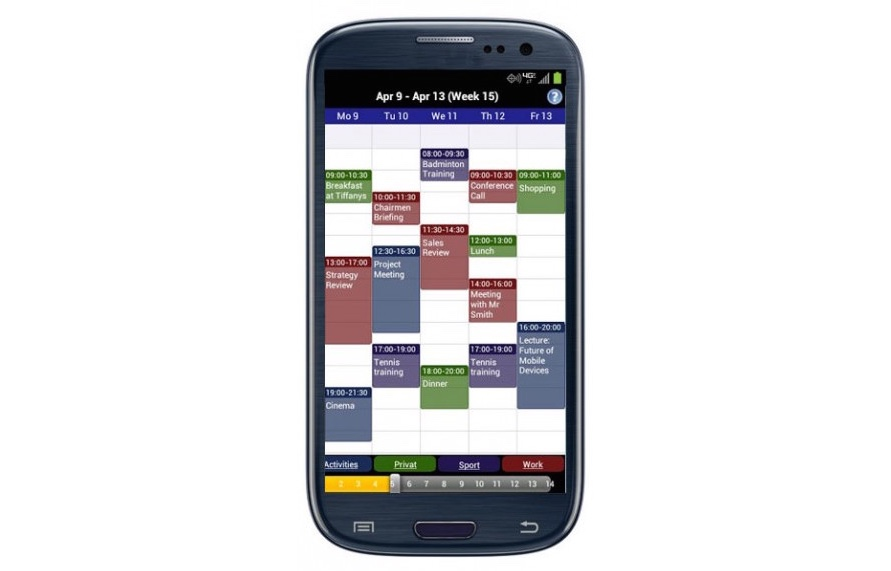
\includegraphics{../img/calendar.jpg}
\caption{Beispiel Kalender Applikation\label{figCalendar}(``Our 10
Favorite Calendar Apps to Keep Your Schedule in Check'')}
\end{figure}

Diese Darstellung eignet sich auch für die geplante
Zeiterfassungsanwendung. ``Events'' eines Tages können wie die
Ereignisse in einem normalen Kalender dargestellt werden.

\textbf{Vorteile:}

\begin{itemize}
\itemsep1pt\parskip0pt\parsep0pt
\item
  Sie zeigt die relativen Unterschiede der Zeiten durch proportional
  unterschiedliche Höhen der einzelnen Blöcke
\item
  Sie kann je nach Spaltenbreite mehrere Tage gleichzeitig darstellen
\item
  Sie ermöglicht dem Betrachter qualitativ festzustellen, wieviel
  Aktivität an einem Tag stattfand
\end{itemize}

\textbf{Nachteile:}

\begin{itemize}
\itemsep1pt\parskip0pt\parsep0pt
\item
  Kurze Events können sehr klein werden - und dadurch auch schwer
  klickbar
\item
  Je nach Breite ist nur sehr wenig Platz vorhanden für Beschriftungen
  oder Details auf den einzelnen Einträgen, bei kurzen Events ist dies
  noch akuter.
\item
  Die Umsetzung einer solchen Darstellung ist vergleichsweise aufwendig
\end{itemize}

\subsubsection{Listen-Darstellung}\label{listen-darstellung}

TODO:

\subsection{Datenquellen für den
Prototyp}\label{datenquellen-fuxfcr-den-prototyp}

Für den Prototyp wurde folgende Systeme zur Anbindung gewählt:

Google Kalender, Redmine (Issues), Github (Events). Obwohl nach der
Umfrage Emails ebenfalls sehr häufig genutzt werden, wurde auf die
Abfrage von Emails verzichtet, da diese schwieriger auszuwerten sind.

\newpage

\section{Umsetzung Prototyp}\label{umsetzung-prototyp}

\subsection{Technologie-Wahl}\label{technologie-wahl}

Für die Umsetzung wurde zwischen nativer Entwicklung auf einer mobilen
Plattform wie IOS, Android oder Windows Phone und zwischen einer
Webapplikation entschieden, welche plattformunabhängig läuft.

Da die Umfrage unter den Mitarbeitern ergeben hat, dass beide
Plattformen signifikant vertreten sind, fiel die Wahl auf eine
Webapplikation. Da manche Mitarbeiter eine dedizierte
Smartphone-Applikation in der Umfrage abgelehnt haben, ist eine
Webapplikation ebenfalls zu bevorzugen, da sie auch am Desktop-Computer,
Notebook, Tablet oder ähnlichem benutzt werden kann.

\subsection{Meteor}\label{meteor}

Die Webapplikation wurde unter Meteor entwickelt, einem
``Full-Stack''-Webframework\footnote{``Full-Stack''-Frameworks decken
  alle Schichten einer typischen Webapplikation ab, d.h. vom Client bis
  zum Server. Häufig können sie dadurch die Datenverbindung vom Client
  zum Server abstrahieren.} in Javascript. Meteor basiert auf einem
reaktiven Programmierparadigma und löst Client-Server-Kommunikation und
Data-Binding\footnote{Data-Binding bezeichnet das Verfahren, das User
  Interface (UI) einer Applikation derart an deren Business Logic (BL)
  zu koppeln, das Änderungen an der BL auf das UI reflektiert werden und
  umgekehrt} auf eine einfache Weise, was den Code sehr expressiv macht
und der Fokus auf die Umsetzung des zu lösenden Problem gesetzt werden
kann. Für eine Konzeptarbeitet hat dies entscheidende Vorteile.

Im September 2014 wurde das Build-Tool von Meteor erweitert, sodass auf
eine einfache Weise Phonegap/Cordova-Container-Applikationen erstellt
werden können. Diese Art von Applikation bündelt eine Webapplikation in
einer nativen Applikation und kann in den Apple App Store, im Google
Play-Store oder den Windows Store gestellt werden. Auf der jeweiligen
Plattform erscheint sie als normale Anwendung. In Anbetracht des Themas
``Entwicklung für Handheld'' ein zusätzlicher, sinnvoller Exkurs.
(``Building IOS and Android Mobile Apps with PhoneGap'')

\subsection{Sprache}\label{sprache}

Meteor wird in JavaScript geschrieben, unterstützt aber auch diverse
JavaScript-Dialekte, wovon CoffeeScript für die Umsetzung gewählt wurde.
Ausschlaggebend dafür war die schlankere Syntax, die bessere Lesbarkeit,
sowie syntaktische Erweiterungen und Abkürzungen (``Syntactic sugar'').
(``Meteor Coffeescript''; ``CoffeeScript (Offizielle Seite)'')

\subsection{Authentifizierung}\label{authentifizierung-4}

Meteor stellt ein einfaches Login-System über OAuth zur Verfügung, es
können Google, Facebook, Github und weitere als Login-Provider definiert
werden. Es wurde Google als Login-Provider gewählt, damit können auch
die Firmen-Logins verwendet werden. Ist die Authentifizierung auf Google
erfolgt, können verschiedene Google-APIs abgerufen werden, im Speziellen
die Kalender-API, welche hier verwendet wurde.

Für die Authentifizierung gegenüber Github, Redmine und der
Controllr-Applikation muss allerdings ein ``Access-Token'' in der
jeweiligen Anwendung erstellt und einmalig in der Anwendung dieser
Arbeit gespeichert werden. Für diesen Zweck und weitere Einstellungen
wurde eine Einstellungs-Seite erstellt, wo der User diese Tokens und
weitere Einstellungen abspeichern kann. Siehe Abbildung
\ref{figSettingsScreen}

\begin{figure}[htbp]
\centering
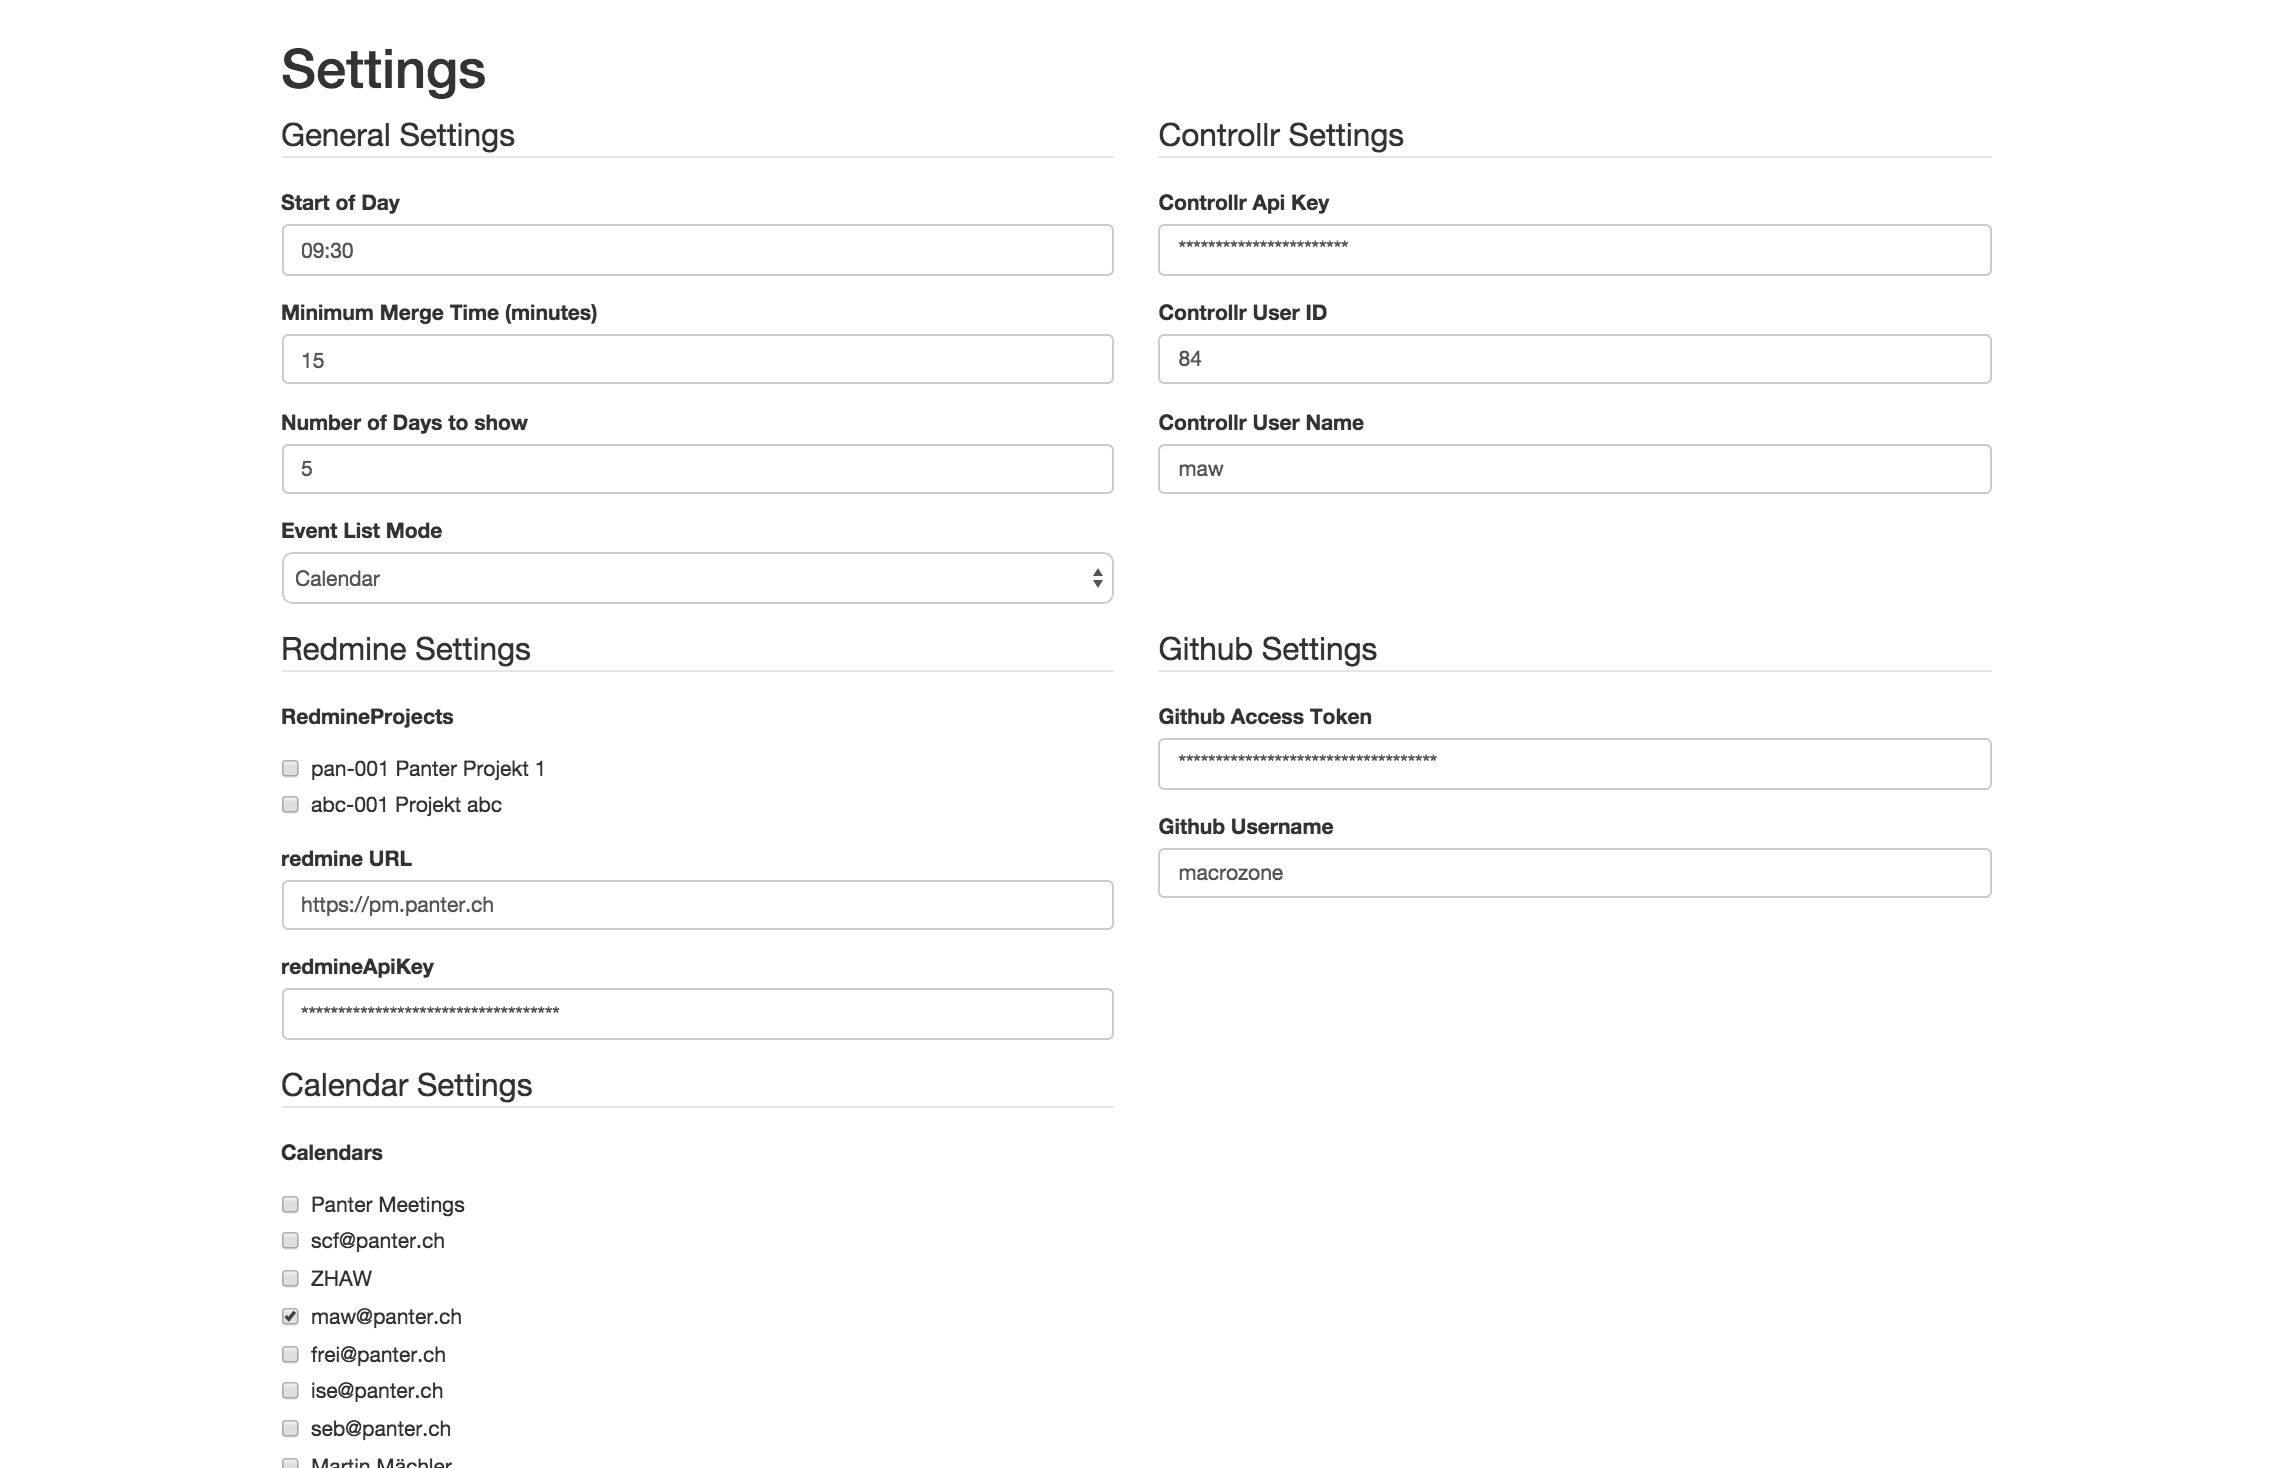
\includegraphics{../img/settingsscreen.png}
\caption{Einstellungs-Bildschrim der umgesetzten
Anwendung\label{figSettingsScreen}}
\end{figure}

\subsection{\texorpdfstring{Reactive-Programming und
REST-Schnittstellen: ``Reactive
REST-Mapping''}{Reactive-Programming und REST-Schnittstellen: Reactive REST-Mapping}}\label{reactive-programming-und-rest-schnittstellen-reactive-rest-mapping}

Meteor implementiert das Programmierparadigma der ``Reaktiven
Programmierung'', dabei werden Änderungen der Datenquellen, welche die
Applikation nutzt, automatisch propagiert und beispielsweise
Darstellungen dieser Datenquellen aktualisiert. (``Reactive Programming
- Wikipedia''; ``Meteor Manual - Transparent Reactive Programming'')

Bei der Umsetzung mussten diverse REST-Apis angesprochen werden. Es
entstand das Bedürfnis, die Zugriffe auf diese REST-APis derart zu
abstrahieren, dass auf dem Client mit normalen Meteor-Collections und
-Subscriptions gearbeitet und dadurch das ``Reactive
Programming''-Modell von Meteor beibehalten werden kann. Dadurch
entstand das ``Smart-Package''\footnote{So werden Pakete von Meteor
  genannt. Pakete können von einer zentralen Registrierungsstelle
  referenziert werden und Abhängkeiten werden automatisch aufgelöst.}
\lstinline!panter:publish-array!, welches in einer initialen Version auf
den Meteor-Paket-Manager gestellt wurde. (``Panter:publish-Array Github
Repository'')

Dieses Verfahren wird nachfolgend ``Reactive REST-Mapping'' genannt.

\lstinline!panter:publish-array! ``publiziert'' ein beliebiges
Javascript-Array aus Objekten auf dem Server als Meteor-Collection auf
dem Client. Dabei muss eine Funktion angegeben werden, welches dieses
Array zurückgibt. In dieser Funktion kann beispielsweise eine REST-API
aufgerufen werden, welche dieses Array zurückgibt. Es kann eine
Intervall-Zeit angegeben werden, wodurch die definierte Funktion
periodisch aufgerufen wird, solange der Client sich auf dieses
Publikation eingeschrieben (``subscribed'') hat.

Durch dieses Verfahren können die Daten aus den verschiedenen Quellen
auf dem Server der Anwendung vorkonsolidiert und vorbearbeitet werden.
Die Daten der verschiedenen ``Event''-Quellen werden beispielsweise in
eine Collection ``Events'' auf dem Client publiziert. Auf dem Client
kann so das normale Data-Binding von Meteor verwendet werden, die
Quellen der Events sind dabei bereits abstrahiert und transparent. Neue
Quellen können somit einfach implementiert werden, der Code für das
Client-UI muss nicht angepasst werden.

\subsection{Verwendete Event-Quellen}\label{verwendete-event-quellen}

\subsubsection{Google Kalendar}\label{google-kalendar}

Meteor verfügt über ein Login-System, welche es ermöglicht, sich
gegenüber Google, Facebook oder weiteren Login-Providern zu
authentifizieren. Wählt man Google als Login-Provider, können auch deren
Schnittstellen abgefragt werden, sofern der Benutzer sein Einverständnis
gibt. (``Meteor Accounts'')

Für Meteor existiert ein Paket \lstinline!percolate:google-api!, welches
den Zugriff auf die REST-APIs von Google erleichtert. Mit Hilfe dieses
Paketes wurden einerseits die Liste der abonnierten Kalender abgefragt,
sowie die Events der gewählten Kalender. (``Meteor Google API'')

\subsubsection{\texorpdfstring{Beispiel für
\lstinline!panter:publish-array! anhand von Google
Kalender}{Beispiel für panter:publish-array anhand von Google Kalender}}\label{beispiel-fuxfcr-panterpublish-array-anhand-von-google-kalender}

Listing \ref{lstGetCalendarList} zeigt ein Beispiel, wie mit dem
erstellen Paket \lstinline!panter:publish-array!, sowie
\lstinline!percolate:google-api! die Liste der abonnierten Kalender
abgefragt und an den Client publiziert wird. (\lstinline!handleIds!
benennt die Feldnamen der IDs um, sodass Meteor-kompatible ID-Felder
zurückgegeben werden (\lstinline!_id!))

\begin{lstlisting}[caption=Publizieren der Google Kalender mit Hilfe von `panter:publish-array` in CoffeeScript, label=lstGetCalendarList]
Meteor.publishArray 
    name: "calendarList"
    collection: "Calendars"
    refreshTime: 10000
    data: (params) ->
        user =  Meteor.users.findOne _id: @userId
        if user?
            url = "calendar/v3/users/me/calendarList"
            result = GoogleApi.get url, user: user
            return handleIds result.items
\end{lstlisting}

Abonniert der Client nun dieses Topic \lstinline!calendarList! mit
\lstinline!Meteor.subscribe("calendarList")!, so steht dem Client eine
Collection \lstinline!Calendars! zur Verfügung, wo alle vom User
abonierten Kalender enthalten sind. Die Collection aktualisiert sich
alle 10 Sekunden, solange der User dieses Topic abonniert hat. Abbildung
\ref{figCalendarSettings} zeigt ein Beispiel, wie es nun möglich, diese
Collection an ein Template zu binden um eine Liste aller Kalender
anzuzeigen. Diese Ansicht wird genutzt, um die Kalender auszuwählen,
welche als Datenquellen verwendet werden sollen.

\begin{figure}[htbp]
\centering
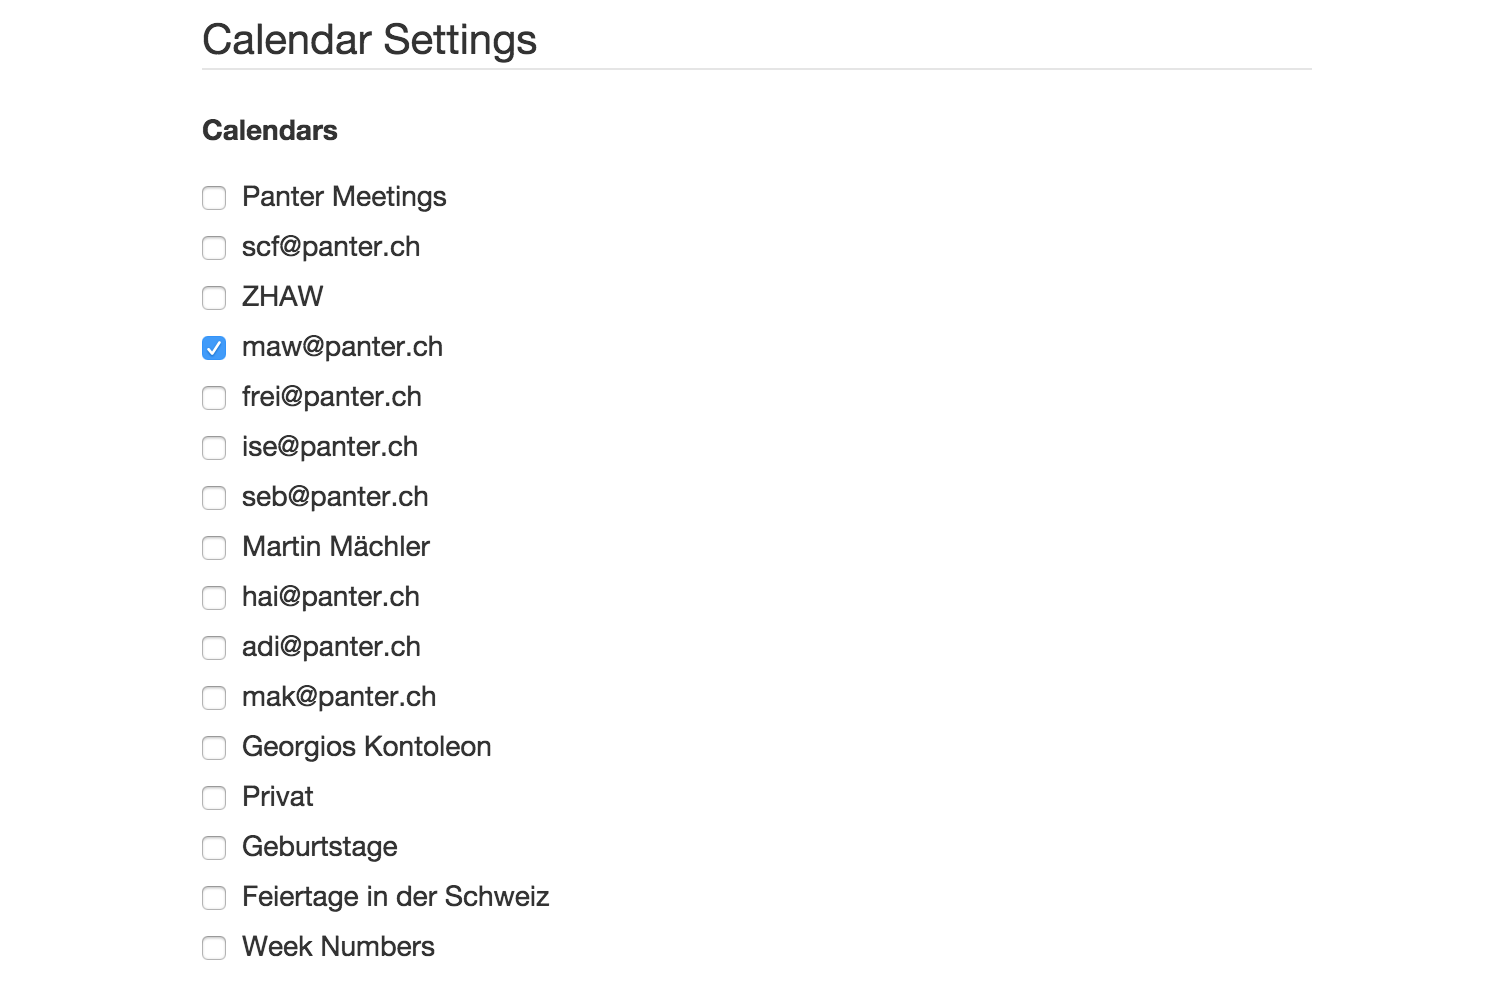
\includegraphics{../img/calendarSettings.png}
\caption{Kalender-Wahl-Bildschrim der umgesetzten
Anwendung\label{figCalendarSettings}}
\end{figure}

Listing \ref{calendarSettingsTemplate} zeigt das Spacebars\footnote{Standard-Template-Sprache
  von Meteor, angelehnt an ``Handlebars'' (http://handlebarsjs.com/)}-Template
des Einstellung-Bildschirms. Dabei wurde das Paket
\lstinline!aldeed:autoform! verwendet, welches es ermöglicht ausgehend
von Schema-Definitionen automatisch Formulare zu erzeugen. (``AutoForm
Github'')

\begin{lstlisting}[caption=Spacebars-Template zur Abbildung \ref{figCalendarSettings}, label=calendarSettingsTemplate]
{{#autoForm collection="UserSettingsStore" doc=settings id="settingForm" type="update" autosave=true}}
  (...)
  {{> afQuickField name='calendars' options=calendars noselect=true}}
  (...)
{{/autoForm}}
\end{lstlisting}

In Listing \ref{claendarSettingsRoute} wird ein Teil der
Routen-Konfiguration des Einstellungsbildschirms gezeigt. Die
Daten-Funktion \lstinline!data! gibt dabei unter anderem ein
\lstinline!calendars!-Feld zurück, welches im Template als Optionen für
das Formularfeld verwendet wird.

\begin{lstlisting}[caption=Routen-Konfiguration für den Einstellungsbildschirm auf Abbildung \ref{figCalendarSettings} in CoffeeScript, label=claendarSettingsRoute]
Router.route 'settings', 
    waitOn: share.defaultSubscriptions
    data: ->
           (...)
        calendars: -> Calendars.find().map (calendar) ->
            label: calendar.summary
            value: calendar._id
        (...)
\end{lstlisting}

Abbonniert nun ein Benutzer einen neuen Kalender auf Google Apps, so
wird innerhalb des Aktualisierungs-Intervals von
\lstinline!panter:publish-array! der neue Kalender geladen und an den
Client publiziert. Auf dem Client wird nun der Einstellungsbildschirm
automatisch um den neuen Kalender ergänzt.

Auf eine ähnliche Art werden die Ereignisse vom Kalender abgefragt und
als ``Events'' publiziert.

\subsubsection{Redmine}\label{redmine-1}

Von Redmine wird die Liste der Projekte geladen, von welchen analog zur
Kalenderliste bestimmte Projekte gewählt werden können, von denen die
Stories und Tasks geladen werden.

Über die issues-Schnittstelle werden die Stories und Tasks geladen, an
denen der Benutzer gearbeitet hat.

\subsubsection{Github}\label{github-1}

Über die ``Events''-Schnittstelle von Github wurden die Aktivitäten des
Users auf Github geladen und als ``Events'' publiziert.

\subsection{\texorpdfstring{Vorteile von ``Reactive
REST-Mapping''}{Vorteile von Reactive REST-Mapping}}\label{vorteile-von-reactive-rest-mapping}

Das Verfahren des ``Reactive REST-Mapping'' wurde über die ganze
Anwendung hinweg gebraucht und erleichterte den Umgang mit den
REST-Schnittstellen sehr. So werden Projekte aus Redmine, ``Issues'' aus
Redmine, ``Events'' aus Github, sowie ``Events'' aus dem Google Kalender
und ``TimeEntries'' aus ``Controllr'' periodisch geladen und alle
Ansichten, welche diese Daten nutzen automatisch aktualisiert.

Ein weiterer Vorteil dieses Verfahren ist, dass die Datenquelle für den
Client völlig transparent ist, der Client ``sieht'' nur gewöhnliche
Meteor-Collections. So lässt sich die Datenquelle oder die
Anbindungs-Technologie einfach austauschen um beispielsweise von einem
``Polling''\footnote{Die Datenquelle wird periodisch abgefragt.} auf ein
Nachrichten-basiertes System zu wechseln, wie es bereits zwischen Client
und Server existiert. Damit entfällt die Verzögerung, die durch das
Polling-Interval entsteht.

\subsection{Event-Darstellung}\label{event-darstellung}

\subsection{Schwierigkeiten}\label{schwierigkeiten}

\newpage
\appendix

\section*{Quellenangaben}\label{quellenangaben}
\addcontentsline{toc}{section}{Quellenangaben}

``AutoForm Github.'' \url{https://github.com/aldeed/meteor-autoform}.

``Building IOS and Android Mobile Apps with PhoneGap.''
\url{https://www.meteor.com/blog/2014/09/15/meteor-092-iOS-Android-mobile-apps-phonegap-cordova}.

``CoffeeScript (Offizielle Seite).'' \url{http://coffeescript.org/}.

``Github Authentifizierung.''
\url{https://developer.github.com/v3/\#authentication}.

``Google Apps Email API.''
\url{https://developers.google.com/gmail/api/v1/reference/}.

``Google Kalender API.''
\url{https://developers.google.com/google-apps/calendar/v3/reference/events\#resource}.

``Google OAuth2.''
\url{https://developers.google.com/accounts/docs/OAuth2}.

``Meteor Accounts.'' \url{https://www.meteor.com/accounts}.

``Meteor Coffeescript.''
\url{http://docs.meteor.com/\#/full/coffeescript}.

``Meteor Google API.''
\url{https://github.com/percolatestudio/meteor-google-api}.

``Meteor Manual - Transparent Reactive Programming.''
\url{http://manual.meteor.com/\#deps-transparentreactiveprogramming}.

``Our 10 Favorite Calendar Apps to Keep Your Schedule in Check.''
\url{http://www.brit.co/10-mobile-calendar-apps/}.

``Panter:publish-Array Github Repository.''
\url{https://github.com/panter/meteor-publish-array}.

``Reactive Programming - Wikipedia.''
\url{http://en.wikipedia.org/wiki/Reactive_programming}.

``Redmine REST API.''
\url{http://www.redmine.org/projects/redmine/wiki/Rest_api}.

``Responsive Webdesign - Wikipedia.''
\url{http://de.wikipedia.org/wiki/Responsive_Webdesign}.

\end{document}
